\chapter{Methods and Methodology}\label{chap_methodology}

The model is implemented in the general-purpose programming language \href{https://www.python.org/}{Python 3} and hosted in \href{https://github.com/}{GitHub}. You can find the repository at \href{https://saguileran.github.io/birdsongs/}{birdsongs}.\\

Today, Python is one of the most widely used programming languages in the world, both by industry and academia. Not only because is easy to learn and write, or because it is popular and used in many fields: websites and software developing, task automation, data analysis, data visualization, server management, or math and scientific computing; it is a highly reliable and efficient language, which allows to user to share and develop code in an easy way due to the supporting of multiple programming paradigms including structured, object-oriented, and functional programming.


\section{Programming Object Oriented (POO)}

POO is more than a way to think about code, it relates to the way  code is created, the software architecture, such that enables flexibility through modular design and maximum reusability. \cite{poo} \\

This programming paradigm offers the user the advantage to easily understanding the operation of a program by gathering data (attribute) and its behavior (method) in a single bundle called an \textbf{object}. Some of the advantages are:

\begin{itemize}
    \item Reusability
    \item Testing and debugging
    \item Flexibility
    \item Speed Up
    
    %\item Easly develop
\end{itemize}

The major disadvantage is that it is a more arduous and labor-intensive process. \cite{poo_coursera}.

\subsection{Python Objects}

\begin{figure}[H]
    \centering
    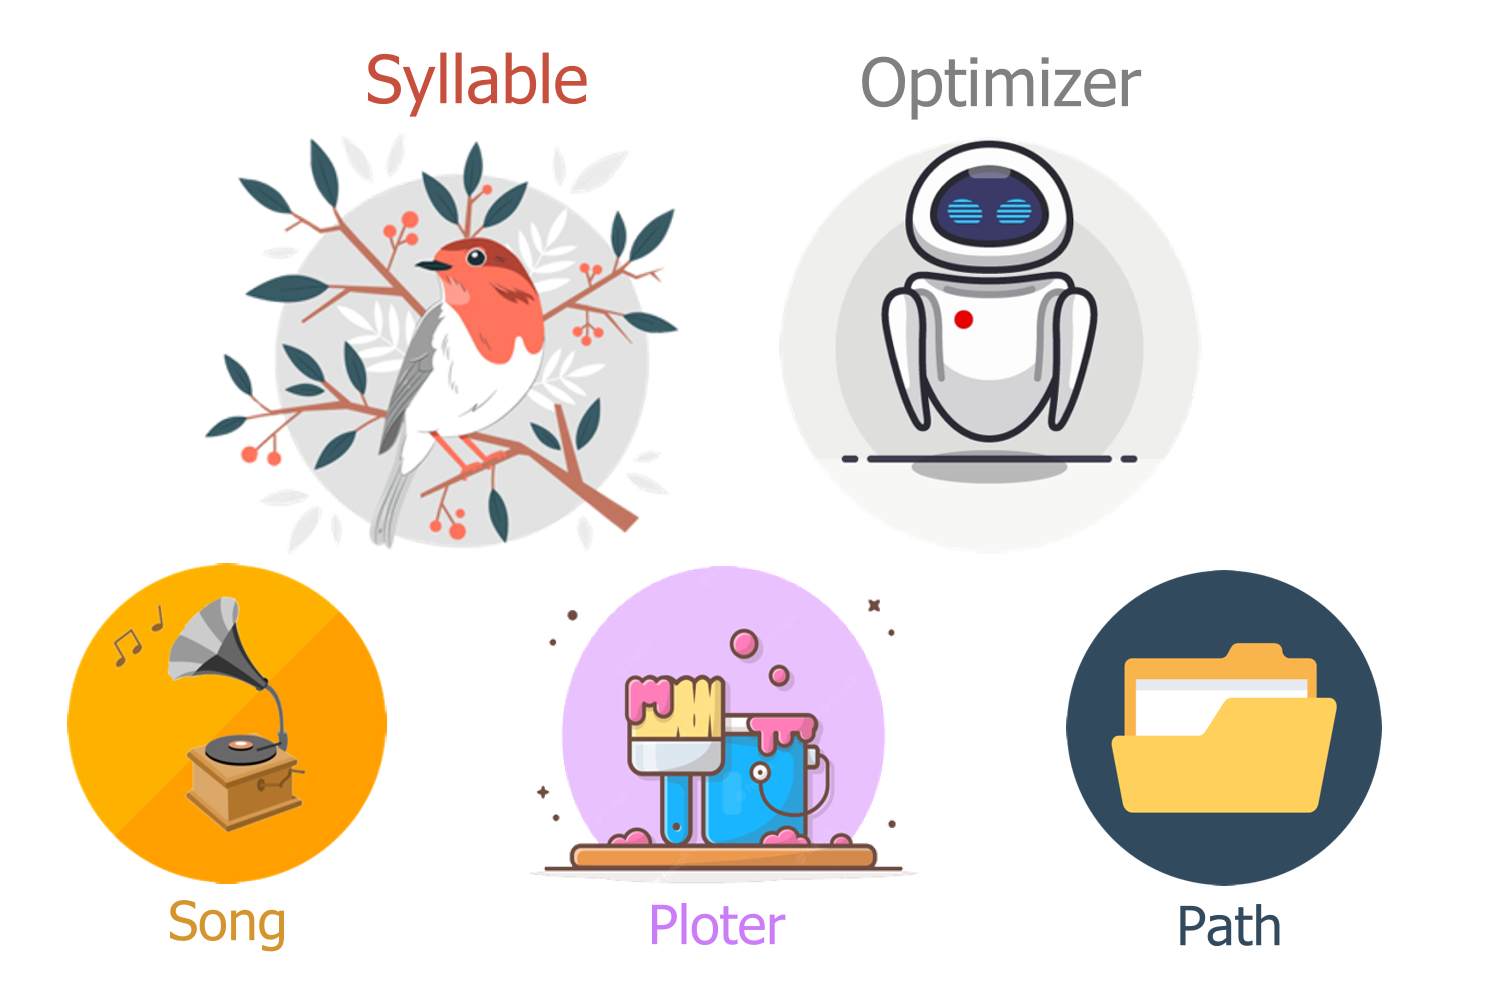
\includegraphics[scale=0.85]{Images/objects.png}
    \caption{Objects created to model, generate, solve, and  visualize synthetic and real birdsongs.}
    \label{fig:objects}
\end{figure}

\section{Model Implementation}

\subsection{Audio Processing}

The signal processing techniques used here are 
\begin{itemize}
    \item Fundamental frequency computing.
    \item Fourier transform.
    \item Signal falterings.
\end{itemize}

they were implemented using the signal processing theory and librosa package \cite{librosa, signal_book_modern}.

\subsection{Methodology}

In order to make the code shareable and public the implementation is made, 

\begin{figure}[H]
    \centering
    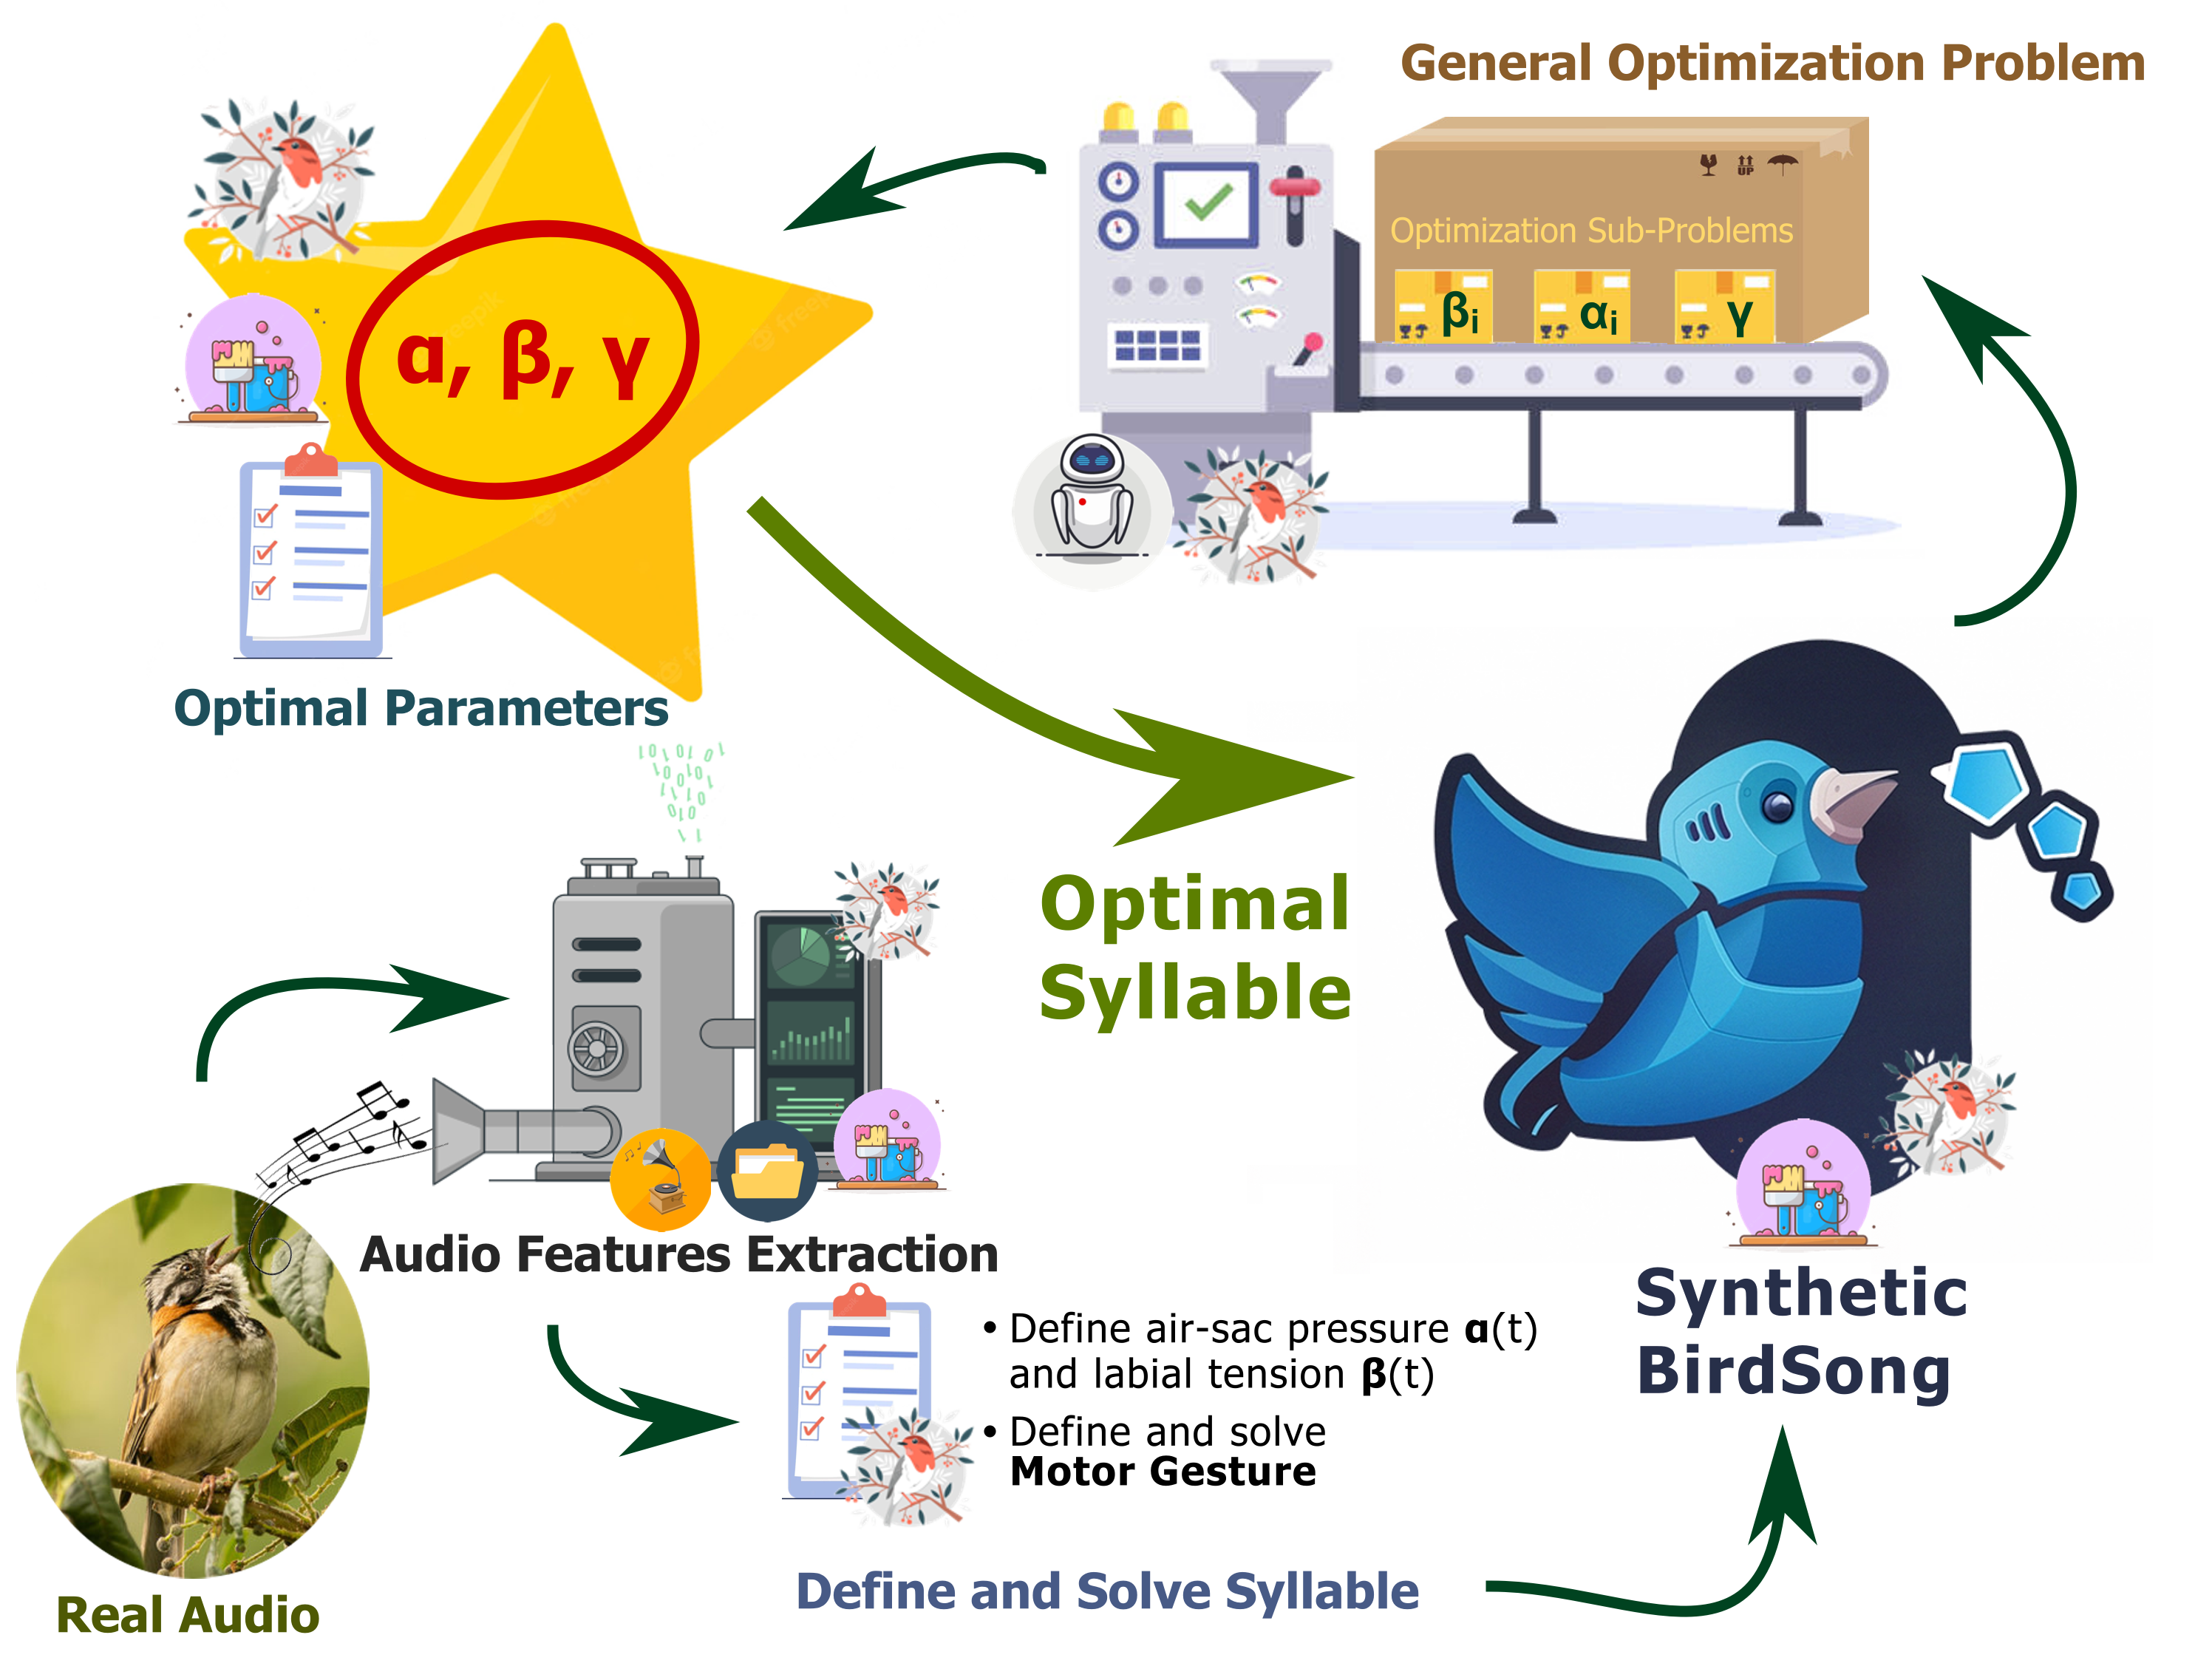
\includegraphics[width=\linewidth]{Images/methodology.png}
    \caption{Schematic programming methodology used to implement and solve the problem.}
    \label{fig:methodology}
\end{figure}



\subsection{Numerical Optimization}

\subsubsection{General Problem}

As was discussed in the previous chapter, the automatization of the model can be summarized to solve the optimization problem defined by the equation \eqref{opt_general}. The major issue of this problem is the parameters space, the optimal solution is in a high dimensional space ($2n+1$) and finding it is a difficult task, and exhaustive and time consuming process since $n$ is usually a huge number. \\

One solution to this drawback is to solve auxiliary optimization problems, each control parameter has its own optimization problem, with lower dimensions. Although this is a good approach to solving the problem, it is still a huge process because the dimensions of the parameters $n$ is still huge\footnote{the size of the control parameters is the same size of the audio signal}.

The solution is to parameterize the control parameters in terms of three or two coefficients for each vector parameter, whichreduces the dimension problem from $2n+1$ to at most $2(3)+1$. 

With these ideas the general optimization problem can be formulated as 

\begin{equation}\label{opt_general_simpl}
\begin{aligned}
\underset{ \gamma \in \mathbb{R},\; a,b\in \mathbb{R}^3}{\text{min}} &\qquad  ||\hat{SCI}_{real} - \hat{SCI}_{synt} ( \gamma,a,b)||_2  + || (\hat{FF}_{real} - \hat{FF}_{synt}(\gamma,a,b)||_2\\
    \text { subject to }  & \qquad \gamma \in \Omega_\gamma, \quad  b \in \Omega_b ,  \quad  a \in \Omega_a
\end{aligned}
\end{equation}

with $\Omega_\gamma = [1000, 100000]$, $\Omega_a=[0.01,0.25]\times[-2,2]\times[0,2]$ and $\Omega_b=[-1,0.5]\times[0.2,2]\times[0,3]$ the feasible regions for each variable. In order to get an objective function dimensionless the following two variables are define

$$
\hat{SCI} := \frac{SCI}{dim(SCI)} , \qquad
\hat{FF}  := \frac{1}{dim(FF)} \frac{FF}{1 \; KHz}
$$

where $dim()$ is the dimension the corresponding vector. \\

To reduce the dimensionality problem, the air-sac pressure and labial tension over the time are parameterized  in term of at most three coefficients, that depends of time, as follows
\begin{gather}\label{eq:alpha-beta_definitions}
\alpha(t) = a_0 + a_1 t + a_2 t^2,  \\
\beta(t) = \begin{cases} 
      b_0  + b_1 \big(\frac{FF_{real}}{10^4}\big) + b_2\big(\frac{FF_{real}}{10^4}\big)^2, \quad \text{id=syllable} \\
      b_0  + b_1 t + b_2 t^2, \qquad \qquad \qquad \;  \; \;  \text{id=chunck}
   \end{cases}
\end{gather}

with the same time duration ($T$) as the input signal, $t\in[0,T]$.

\subsubsection{Optimization Sub-problems}

The general problem is computationally expensive since it still depends on several variables. Although solving the problem all at once is the ideal method, a better approach is to divide it into three auxiliary problems, one optimization problem for each control parameter.

\begin{itemize}
\item  \textbf{Optimal Time Scaling Constant ($\gamma$)}

The time scaling coefficient parameter ( $\gamma$) should be the same for all syllables of the same song, in general a bird has the same $\gamma$ value for all its syllables. This parameters modifies the spectral content, increasing or decreasing it, so to find its optimal value the following optimization problem must be solved
\begin{equation}\label{eq_optimal_gamma}
\begin{aligned}
\underset{ \gamma \in \mathbb{R}}{\text{min}} &\qquad   || \hat{SCI}_{real} - \hat{SCI}_{synt} ( \gamma)||_2  + || \hat{FF}_{real} - \hat{FF}_{synt}(\gamma)||_2\\
    \text { subject to }  & \qquad  \;   \gamma \in \Omega_\gamma = [10000, 100000]
\end{aligned}
\end{equation}

In this auxiliary problem the other control parameters ($\alpha$ and $\beta$) are taken constant but ensuring they are in region of oscillations defined by the bifurcation theory, the feasible region is defined by the analyze of parameters behavior of previous works.

\item  \textbf{Optimal Air-Sac Pressure ($\alpha$) Coefficients}

The parametric coefficients of the air-sac pressure ($\alpha$) are calculated by solving the following maximization problem 

\begin{equation}\label{optimal_a_max}
\begin{aligned}
\underset{a \in \mathbb{R}^3}{\text{max}} &  \qquad corr (real, synthetic(a))  \\
    \text { subject to }  &  \qquad \;  a \in \Omega_a
\end{aligned}
\end{equation}

This is done by computing the acoustic dissimilarity between the coefficients of the real and synthetic spectrums, this set of coefficients has the information of the harmonic of the audio signal. Then, the dissimilarity correlation is an appropriated objective function to solve the search for the optimal parameters for the air-sac pressure, remember that this control parameter impacts the intensities and distances of the harmonics of the signal.\\

As every maximization problem is equivalent to solve the a minimization problem, instead of solving the problem \eqref{optimal_a_max} we will solve the following minimization problem
\begin{equation}\label{optimal_a_min}
\begin{aligned}
\underset{a \in \mathbb{R}^3}{\text{min}} &  \qquad - corr (real, synthetic(a))  \\
    \text { subject to }  & a\in\Omega_a
\end{aligned}
\end{equation}

where the feasible region, $\Omega_a = [0, 0.25] \times [-2,2] \times [0,2]$, is defining by the study and exploration of the model and its bifurcation theory.

\item \textbf{Optimal Labia Tension ($\beta$) Coefficients}

The last step is to find the parametric coefficients of the labial tension $b_i$. Since the labial tension is the key player in the sound production of birds, as it modulates the air at certain frequencies, the fundamental frequency is highly dependent on this control parameter. Therefore, a good objective function should include this spectral variable. \\

The optimization problem defined to find the optimal parameters of the labial tension is
\begin{equation}\label{optimal_b}
\begin{aligned}
\underset{b \in \mathbb{R}^3}{\text{min}} &\qquad || FF_{real} - FF_{synt} (b)||  \\
    \text { subject to }  & \qquad \; b \in \Omega_b
\end{aligned}
\end{equation}

where the feasible region is $\Omega_b = [-1,0.5]\times[0.2,2]\times[0,3]$
\end{itemize}

At present, there are many algorithms and packages created to solve any type of optimization problem, from linear to nonlinear\footnote{Soome lirabries as \href{https://web.casadi.org/}{CasaADI}, \href{mathworks.com/products/optimization.html}{Matlab optimization toolbox}, of lmfit \cite{lmfit}}.
Because the model was implemented in Python and after a literature review, the most appropriated library to solve the optimization problems presented in this work is the Non-Linear Least-Squares Minimization and Curve-Fitting for Python (lmfit \cite{lmfit}), which is both a powerful and easy to use.
